% $Id: AdmitDesign.tex,v 1.43 2015/04/02 21:25:59 rauch Exp $

\documentclass[preprint]{aastex}
\usepackage{epsfig}
\usepackage{graphicx}
\usepackage{float}
\usepackage{fancyvrb}
\title{ADMIT Design Overview\\
\today
}
\begin{document}
\maketitle

\section{Introduction}\label{s-intro}

The ALMA Data Mining Toolkit (ADMIT) is a value-added software package
which integrates with the ALMA archive and CASA to provide scientists with
quick access to traditional science data products such as moment maps,
and with new innovative tools for exploring data cubes and their many
derived products. The goals of the
package are to (1) make the scientific value of ALMA data more immediate
to all users, (2) create an analysis infrastructure that allows users to
build new tools, (3) provide new types of tools for mining the science in
ALMA data, (4) increase the scientific value of the rich data archive
that ALMA is creating, and (5) re-execute and explore robustness of
the initial pipeline results.

For each ALMA science project a set of science quality image cubes
exist. ADMIT runs a series of ``ADMIT tasks,'' which are essentially
beefed up CASA tools/tasks, and produces a set of Basic Data Products
(BDP).  ADMIT provides a wrapper around these tasks for use within the
ALMA pipeline and to have a persistent state for re-execution later on by
the end user in ADMIT's own pipeline.  ADMIT products are contained in
a compressed archive file {\it admit.zip}, in parallel with the existing
Alma Data Products (ADP)\footnote{Examples of ADP in a project are the
Raw Visibility Data (in ASDM format) and the Science Data Cubes (in FITS
format) for each target (source) and each band}.

Once users have downloaded the ADMIT files, they can preview the work
the ALMA pipeline has created, without the immediate need to download the
generally much larger ADP. They will also be able to re-run selected portions
of the ADMIT pipeline from either the (casapy) commandline, or a
(CASA) GUI, and compare and improve upon the pipeline-produced
results. For this some of the ADP's may be needed.

\section{ADMIT Tasks} \label{s-at}

An ADMIT Task (AT) is made up of zero or more CASA tasks.  It takes as
input zero or more BDPs and produces one or more output BDPs.  These BDPs
do not have to be of the same type. An AT also has input parameters that
control its detailed functionality. These parameters may map directly to
CASA task parameters or may be peculiar to the AT.  On disk, ATs are stored
as XML. In memory, each is stored in a specific class representation derived
from the ADMIT Task base class.  A user may have multiple instantiations
of any given AT type active in an ADMIT session, avoiding need to to save
and recall parameters for different invocations of a task.  The workflow
manager (section \ref{s-workflow} keeps track of the connection order of
any set of ATs.   AT parameters are validated only at runtime; there is
no validation on export to or import from XML. The representations of
every AT are stored in a single XML file (admit.xml).

\section{Basic Data Products} \label{s-bdp}

Basic Data Products are instantiated from external files or created as
output of an ADMIT Task.  As with ATs, the external data format for BDPs
is XML and in memory, BDPs are stored in a specific class representation
derived from the BDP base class.  One XML file contains one and only one
BDP.  When a BDP is instantiated by parsing of its associated XML file,
the file first undergoes validation against a document type definition
(DTD).  Validation against a DTD will ensure that the XML nodes required
to fully instantiate the BDP are present.  Since BDP types inherit from
a base class (see Figure \ref{admitarchitecture}), there is a BDP.dtd
which defines the mandatory parameters for all BDPs. For each BDP type,
there is also a DTD that defines parameters specific to that BDP type.
Individual BDP Types are described in Section \ref{s-bdptypes}.

The DTDs for each BDP type will have been autogenerated directly from the
class definition Python.  Furthermore, the DTD is included in the XML file
itself so that the BDP definition is completely self-contained.  The ensures
integrity against future changes to a BDP definition (i.e., versioning).
To allow for flexibility by end users (aka ``tinkering''), extraneous nodes
not captured in the DTD will be ignored, but will not cause invalidation.
Validation against the DTD happens ``for free'' with use of standard XML
I/O Python libraries.  Data validation occurs on both write and read.

A typical BDP instantiation from XML looks like:

\begin{verbatim}
import parser
b = parser.Parser("myfile.xml")
\end{verbatim}

\noindent {\it Parser} is a class that uses the SAX library to interpret the
XML contents.  Inside the XML is a {\it BDPType} node that indicates
the BDP derived type stored in the XML file, which will be returned
by the call. This is essentially the factory design pattern.
The XML parser converts a member datum to its appropriate type, then 
assigns the datum to a variable of the same name in the class.
For example:
\begin{verbatim}
<noise type="Float">3.255</noise>
\end{verbatim}
is converted to
\begin{verbatim}
BDP.noise =3.255
\end{verbatim}
\noindent
In serializing the BDP, we use Python introspection to determine the
variable names and data types and write them out to XML, essentially
reversing the process.  Individual BDP Types are described in
Appendix \ref{s-bdptypes}


\section{Workflow Management}\label{s-workflow}

We take an task-centric view of workflow in which an ADMIT Task (AT)
is an arbitrary M-to-N mapping of BDPs, possibly with additional
internal attributes and methods.  BDPs are passive
data containers, without parents or children, and are owned by the AT
which produces them. Hence, ATs also function as BDP containers.
The Flow Manager (FM) maintains a full list of ATs and how they are
connected, allowing it to keep all BDPs up to date as ATs are modified.

Conceptually, a connection maps the output(s) of one AT to the input(s) of another AT. The Flow Manager creates an overall connection map, where a single 
connection is specified by a six-element element tuple of integers indices: 
$$
({\rm project_{out},AT_{out},BDP_{out},project_{in},AT_{in},BDP_{in}}).
$$

\noindent In most cases, the input project and output project will be the 
same, but in the case of virtual projects they can differ.
Figure \ref{connection} illustrates the connection map concept,
while Figures \ref{flow6-AT} and \ref{flow6-FM} give an realistic example workflow and the resulting connection map.
\begin{figure}[H]
\begin{center}
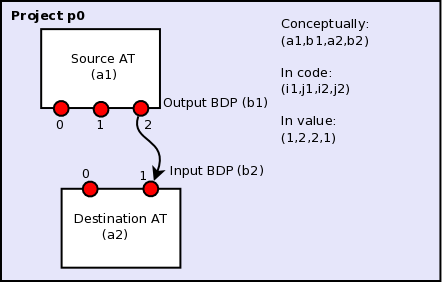
\includegraphics[scale=0.5]{connection.png}
\end{center}
\caption{The connection in this diagram connects two ATs, {\it a1} and
{\it a2},  inside a single project {\it p0}.   The output BDP of {\it a1}
is an input BDP of {\it a2}, i.e. $b1 \equiv b2$.   A given output BDP
may be the input to an arbitrary number of ATs, but can be the
output one and only one AT.   For virtual projects, the first and fourth
indices in the tuple, $i1$ and $i2$, would differ.
}
\label{connection}
\end{figure}
\clearpage

\begin{figure}[H]
\begin{center}
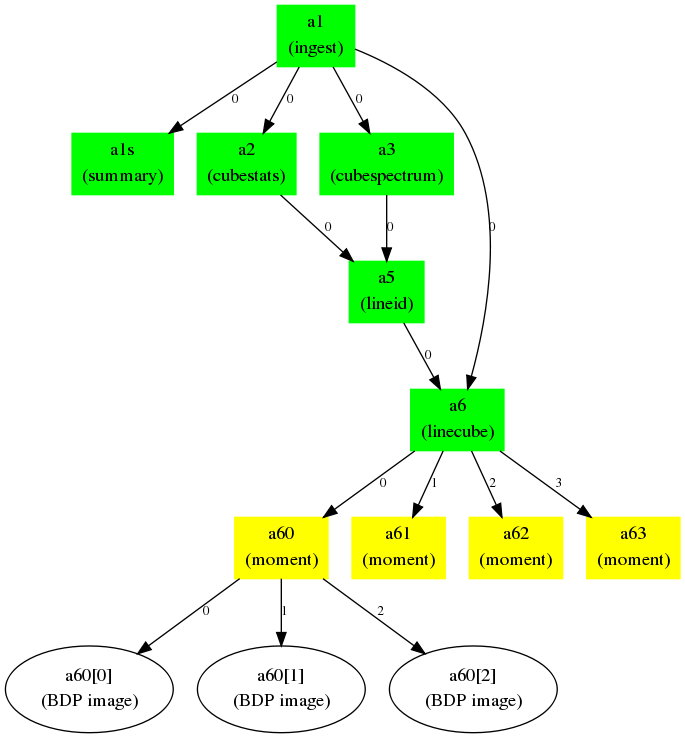
\includegraphics[scale=0.7]{flow6-AT.png}
\end{center}
\caption{Example realistic workflow with task connection map. A FITS cube is
ingested (a1) and processed through a number of tasks: summary,
statistics, spectral line cut out, moment. Integers along the arrows
indicate the output BDP index available to the next task in the map.}
\label{flow6-AT}
\end{figure}

\begin{figure}[H]
\begin{center}
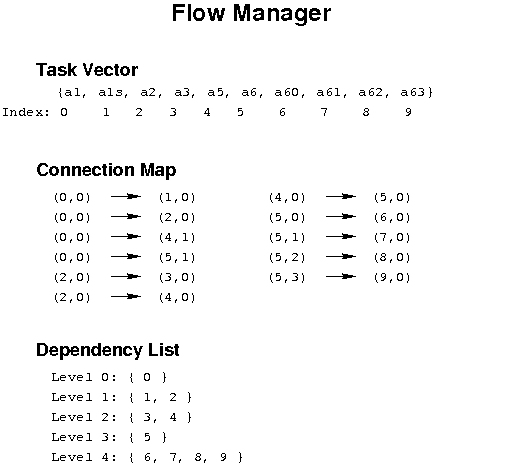
\includegraphics[scale=1.1]{flow6-FM.png}
\end{center}
\caption{The Flow Manager connection map and dependencies for the workflow
in Figure \ref{flow6-AT}. The tuples in the connection map give the
project, ADMIT task, and BDP output/input indices. The Flow Manager also
computes the dependence list of ATs so that a change in one AT will trigger
re-execution of ATs that depend on it in order to recompute the BDPs.}
\label{flow6-FM}
\end{figure}


\clearpage


\section{Architecture Overview}\label{s-arch}


Figure \ref{admitarchitecture} is a schematic of the overall interaction
of ADMIT modules. Their functionality is described below.

\begin{figure}[H]
\begin{center}
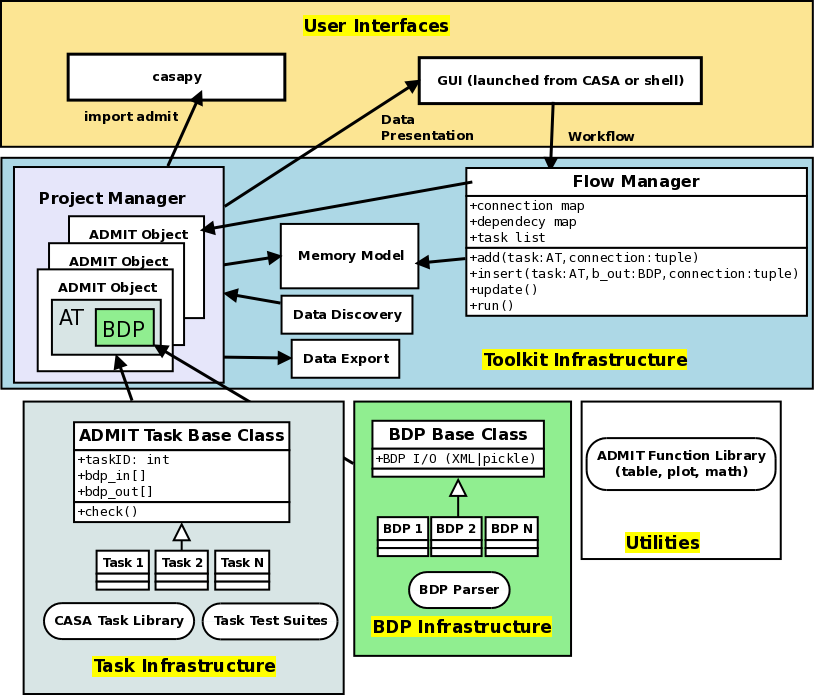
\includegraphics[scale=0.45]{AdmitArchitecture.png}
\end{center}
\caption{ Schematic of how ADMIT fits together. }
\label{admitarchitecture}
\end{figure}


\subsection{BDP Infrastructure}

The BDP Base Class contains methods and member variables common to all BDPS.
Individual BDPs derive from it and add their own special features.  BDP I/O
is built-in to the base class through Python XML libraries.

\subsection{Task Infrastructure}

\begin{itemize}
\item {\it ADMIT Task Classes} - An ADMIT Task Base Class allows one or
more CASA tasks to be encapsulated within one ADMIT Task.  The base class
should indicate required methods and member variables such that a user
can write her own AT.  Individual ADMIT Tasks derive from the ADMIT Task
Base Class.


\item {\it Task Test Suites} - Each Task must have at least a unit test and integration test.

\item {\it CASA Task library }  - From which ADMIT tasks may be built.

\end{itemize}

\subsection{Utilities}
This ADMIT Function Library includes useful generic classes to handle
tables, plotting, and mathematical functions. Utilities will expand
as needed.

\subsection{Toolkit Infrastructure}

\begin{itemize}
\item {\it Data Discovery/Export/Import} - This is the module that examines
the working directory recursively for FITS files and ADMIT products.
It should be able to recognize vanilla, ALMA-style, and VLA-style directory
trees and branch accordingly.  It will also handle the case of giving
a self-contained subset of ADMIT products to a collaborator. It would
write a single compressed file containing the ADMIT products in the
appropriate hierarchy.  

\item {\it ADMIT Object} - From the results of data discovery, 
the an ADMIT object is instantiated in memory as well as setting up
the initial workflow for an ADMIT run (or re-run).  This initialization
includes instantiation of any discovered ATs and BDPs.  One ALMA project
maps to one ADMIT object.

\item {\it Memory Model} - How the ADMIT object and state are kept up to date.
This is a combination of the Admit Object(s) and the Flow Manager state.
The memory model has a one-to-one mapping to what's on disk.

\item {\it Flow Manager } - This is the infrastructure that
strings Tasks together, manages the connection map, decides if ATs and
BDPs are out of date and need to be re-run, and manages ``task branches.''  

\item {\it Project Manager } -  The PM is a container for one or more
ADMIT objects, sometimes referred to as a {\it virtual project}.  The PM
allows for data mining across different ALMA projects.  

\end{itemize}


\subsection{User Interfaces}
\begin{itemize}
\item {\it casapy} - For scripting or direct AT invocation, CASA will be
the supported environment.  ADMIT specific commands enabled
by ``import admit''. There is also the {\tt \#!/usr/bin/env casarun}
type environment.


\item {\it Graphical User Interface} - The GUI will invoke the ADMIT
pipeline via the GUI-Python interface as well as present data and Task
interfaces to the user, and allow construction of workflows.  {\bf Still
to be designed} 
\end{itemize}
\clearpage



% -- Maybe use this somewhere. --
%Photo processing tools such as Adobe's LightRoom and the open source
%DarkTable follow this model.  They use a style to define a template how
%the photo is to be processed, we will use something similar (see below)
%to ease the use of ADMIT via pre-defined meta-procedures (flow procedures?).


\section{ALMA archive tree}

This archive tree is still under flux, here are some actual examples
of the Project/Sgous/Gous/Mous (P/S/G/M) hierarchy as can be found when a user
unwinds their tar file:\footnote{different targets (T) can be found inside of the
P/S/G/M hierarchy....}


%  du | awk '{print $2}' | sort | sed s,./,, > log1

\footnotesize
\begin{verbatim}

2012.1.00001.S/                                     # P: project [1]
   science_goal.uid___A002_X5a9a13_X7ab/            # S: "sgous"
      group.uid___A002_X5a9a13_X7ac/                # G: "gous"
         member.uid___A002_X5a9a13_X7ad/            # M: "mous" [5]
            calibration/
            log/
            product/                                # TBD: product/product/science/...
               foobar.fits                          # SPWcube (+ foobar.flux.fits)
               foobar.admit/                        # our ADMIT tree [2]
                  admit.xml
                  foobar.cim/                       # working CASA Image cube (~foobar.fits)
                  cubestats.bdp                     # cube statistics
                  linecube.13CO-110.201/            # line cube ID'd as 13CO(1-0)  [4]
                      linecube.13CO-110.201.mom0    # 13CO moment map [1]
                      cubestats.bdp                 # 13CO cube statistics
                  linecube.CO-115.271/              # line cube ID'd as 12CO(1-0)
                      linecube.U-115.271.mom0       # 12CO moment map
                      cubestats.bdp                 # 12CO cube statistics
                   linecube.U-112.268/              # an unidentified line
                      linecube.U-112.268.mom0       # moment map
                      cubestats.bdp                 # cube statistics
               foobar.zip                           # lightweight export version of foobar.admit [3]
            qa/
            raw/
            script/
         member.uid___A002_X5a9a13_X7af/            # next "mous" in this "gous"
            ...            
\end{verbatim}

\noindent
{\bf Notes:}

\begin{enumerate}

\item From the top level this hierarchy covers 8 directories deep

\item Each spectral window cube {\tt foobar.fits} (with optionally a {\tt foobar.flux.fits} for PB correction)
results in a {\tt foobar.admit} working directory with a single {\tt admit.xml} file

\item Lightweight export ADMIT Objects will be called {\tt foobar.zip}

\item Each Line Cube results in a sub-directory within which analysis of that cube takes place

\item Only a {\tt mous} product tree is shown here, but there will also be one at the {\tt gous} level

\item Different targets (``sources'') are not described here yet, because your author has no clue yet where they go. 
\end{enumerate}

\normalsize


\subsection{Graphical User Interface}

The graphical user interface will be designed and implemented in year
2. There are technical decisions to make such as whether ADMIT would
benefit from a zoomable user interface, whether we should stick with Qt
toolkit since that's what CASA uses, etc.


\appendix 

\section{Example Code}

This is working example that ingests a FITS file, makes moments, saves the
ADMIT state, restores it, modifies the moment parameters and then remakes 
the moments.

\fvset{numbers=left,fontsize=\small
%,samepage=true
}  
\VerbatimInput{../admit/test/milestone1.py}

\section{Remaining Questions}


A still random list of things we should prioritize on when and where they go in ADMIT:

\begin{enumerate}

\item Deal with removal of BDP data files ``outside the sandbox" - should trigger stale=True.  
This does not include removal of XML files which breaks the contract.  
Doug is writing a AT.missingFiles() method.


\item
usage of CASA Tasks vs. Tools.  Using a number of tools can be more efficient,
and this can make one wonder if in a flow, where the tools are repeatedly
instantiated in tasks, it could benefit from keep that cached?

\item
When a user like a certain AT, but wants to add another control parameter.
We should make it easy to create a tear-off version of the AT.

\item
Stuff away other useful info about objects (e.g. from NED, or Sloan,
or somewhere), for later data mining. This is more for once the projects
are locally managed.

\item
Ensure WCS sanity in case where image coordinates are used (instead of
dra/ddec, or ra/dec)

\item
FREQ or VELO axes should work equally well.
%Line detections can perhaps be skipped in VELO cases?

\item
Do we need a multi-access BDP?  In the current thinking a BDP is read-only
once created.  But like in miriad images, a header can be changed.
Or where do we store/change keywords/info/containers for a BDP once it
has been created.

\item
Pipeline parameters from different AT/BDP linked to ADMIT for easier
personalized overview while re-running pipeline. This is something for
the GUI especially.

\item
What to do about intermediate results that are normally discarded. If they
are a BDP, the pipeline might recompute them?  Need special tag that's
ok to be absent unless needed down the pipe?  Or force scripts to keep
them inside of an AT.?

\item
What files can be missing from the BDPs. Can we use line cube's and not
need the big band cube?

\item
How to verify data are what they are in the archive when
recomputed. checksum is dangerous, and likely to give false positives due
to roundoff and optimized code.  differencing the JPG or PNG might work as
a first indication, but the real verification isn't until the real big data
is downloaded and difference histogram verified? isn't there a better way?

\item 
What really goes into the archive

\item
polarization (IQUV, XX,YY,...,  LL,RR,...)

\item
Is there a good use for pickle to move to another better equipped ipython
(other than numpy, scipy and matplotlib) and continue data analysis/mining
there? Or can CASA's ipython bridge to a modern ipython/notebook?

\item 
How to handle absorption lines? See for example the Sgrb2 test data.

\item
How to handle LineCube's with blended lines. Should sphisticated masking
with PPV split them?  That requires feature identification, and we don't
have this available yet at the LineCube stage. Iterate one more time via
the cube?


\end{enumerate}


\section{BDP Types}\label{s-bdptypes}
\input BDP/Summary
\input BDP/CubeSum
\input BDP/CubeSpectrum
\input BDP/CubeStats
\input BDP/Moment
\input BDP/ContinuumMap
\input BDP/SPWCube

\input BDP/LineList
\input BDP/LineCube
\input BDP/PVSlice
\input BDP/PVcorr
\input BDP/PeakPointPlot
\input BDP/SpectralMap

\input BDP/OverlapIntegral
\input BDP/DescriptionVector
\input BDP/FeatureList

\clearpage

\section{Individual AT Designs}\label{s-atdesign}
\input AT/example
\input AT/File
\input AT/Flow
\input AT/Ingest
%\input BDP/Summary
%\input BDP/CubeSum
\input AT/CubeSpectrum
\input AT/CubeStats
%\input AT/Moment
%\input BDP/ContinuumMap
%\input BDP/SPWCube

%\input AT/LineList  is now LineID
\input AT/LineID
\input AT/LineCube
\input AT/PVSlice
\input AT/PVCorr
%\input AT/PeakPointPlot
%\input AT/SpectralMap    % deprecated, absorbed into 

%\input BDP/OverlapIntegral
%\input BDP/DescriptionVector
%\input BDP/FeatureList


\section{Glossary}

\begin{itemize}

\item {\bf ADP} 
see: {\it ALMA Data Product}



\item {\bf ALMA}
A bunch of fancy radio telescopes in a high and dry desert. There are some 12m dishes
and some 7m dishes for interferometry, and a few total power dishes for on-the-fly
single dish mapping. % need some numbers 

\item {\bf ALMA Data Product}  A term we coin here, to differentiate from our ADMIT BDPs.

\item {\bf ADMIT}

\item {\bf ADMIT object} Reference to the ADMIT data that describe a FITS cube. This is
either a directory, within which ADMIT has placed various derivates, or a lightweight
ZIP file, which can be ingested in the ALMA Science Archive. Users can take this ZIP
file and quickly recreate an ADMIT flow.


\item {\bf ADMIT Task}
(AT) is a lightweight python wrapper performing basic ADMIT tasks. Implementation
can be using CASA, or other packages such as MIRIAD or NEMO. Needs input
and output BDPs, and control is via a defined set of keyword-value pairs
that persist with the stored BDPs for re-computation.

\item {\bf AT}
see: {\it ADMIT Task}


\item {\bf BandCube} 
An image data cube convering a single ALMA BAND (usually 1.5 GHz). This is
the default mode of data delivery, users will get up to 4 bands if they all contain science goals.
See also {\bf SPWCube} 

\item {\bf Basic Data Product}
Lightweight XML wrapper around ADMIT basic data, such as data images and cubes, and tables. a BDP also
stores which other BDP it depends on, and which BDPs depend on it, and the task with which it was
created and the associated task parameters. This ensures that a workflow can be recomputed and braught
back up to date.

\item {\bf BDP}
see: {\it Basic Data Product}

\item {\bf CARTA}
Visualization system developed for CASA/ALMA. Replacing the viewer.

\item {\bf CASA}
Python based data reduction system for ALMA and VLA data (and maybe more). Data are stored
in tabular format, which are directories.

\item {\bf FITS}
is a file format used to store multidimensional (up to 7) data cubes. For ADMIT
the normal starting point are FITS images or cubes, although the ingestion

\item {\bf flow}
In ADMIT we talk about a {\bf flow}, much in the same way as {\it pipeline} is 
often used in other contexts. We want to differentiate here, because we can create
links between flows and make them depend on each other.

\item {\bf FlowManager}

\item {\bf GOUS}  Part of the ``P/S/G/M'' hierarchy in ALMA data products.

\item {\bf ingestion}
This is normally the first step ADMIT takes : a FITS file is converted to an internal format
that the package that ADMIT is using (normally a CASA Image).

\item {\bf line}
The word ``line'' is often used to refer to a Molecular Line or Line Transition
that ADMIT attempts to identify and isolate from the SPWcube.
We have ADMIT products such as {\it LineList} and {\it LineCube}.
The ADMIT pipeline encodes line names (optionally) in the filename, once lines have 
been identified.  Examples are for CO(1-0) would be {\tt CO-115.27} and 
N$_2$H$^+$ would be {\tt N2HP-93.17}. Unidentified lines will go by
names such as {\tt U-98.75}.


\item {\bf MIRIAD}
is a radio interferometry data reduction package,
used by BIMA, CARMA, SMA, WSRT, ATCA and maybe others.  Unix command line,
keyword=value command line interface, the -k and -kw arguments provide inline
help. Handles visibiity data and image, does calibration, mapping and image
analysis.

\item {\bf MOUS}  Part of the ``P/S/G/M'' hierarchy in ALMA data products.

\item {\bf NEMO}
Stellar dynamics toolbox, but since it handles images and fits, can also be used for
portions of an analysis pipeline.  Unix command line, keyword=value command line interface, 
files can be piped using in=- or out=-. The --help or help=h provide inline help.

\item {\bf Project} At the top level ALMA organizes data in projects. Also known
as the ``P'' in the ``P/G/G/M'' hierarchy.
Hierarchies below this are the SGOUS, GOUS and MOUS. 

\item {\bf SGOUS}  Part of the ``P/S/G/M'' hierarchy in ALMA data products, the Science Goals.

\item {\bf SPWCube} Spectral Window Cube, see {\it BandCube}.

\item {\bf Target} Another (better?) name for Source, more commonly used in ALMA context.
In the ``P/S/G/M'' hierarchy of ALMA data products, you can find multiple targets
below the MOUS and GOUS levels? (to be confirmed).


\end{itemize}





\end{document}

%%%%%%%%%%%%%%%%%% EVERYTHING AFTER THIS IS IGNORED %%%%%%%%%%%%%%%%%%%%%%%
\subsection{Top Level}

Here is a very simple example, finding all FITS cubes in a directory
hierarchy, each {\tt foobar.fits} will have a parallel directory {\tt foobar.admit}
(or read from that directory if it already existed)

\footnotesize
\begin{verbatim}

import admit

# find fits files locally down from here
ff = admit.ADMIT.discover(mode='ALMA',rootdir='.')

for f in ff:                           # loop over all fits found 
   a = admit.ADMIT(f)                  # new admit object
   a.plotmode(0,'png')                 # set a plotmode
   a.pushd()                           # change directory here
   if a.new():                         # a new admit?
      a.pipeset('pickle=1')            # global parameter
      a.pipeset('maxline=0')           # global parameter
      a.pipeset('cubestats/robust=1')  # module parameter
      a.pipeset('moments/sigmaclip=3') # module parameter
      a.pipeload('cubestats,moments')  # construct a pipeline
   a.piperun()                         # run it
   a.pdump()                           # save it (XML/BDP/Pickle)
   a.popd()                            # pop back the directory
   del a                               # optionally delete the object

\end{verbatim}
\normalsize

The {\tt pipeload()} function sets the pipeline flow based on a number
of templates. Common ones are:

\begin{enumerate}
\item[1.] {\it cubestats}:
produces a Summary (always done) and CubeStats
(which also implies a CubeSpectrum). A CubeSpectrum can be expanded
to a SpectralMap by the user. This is probably the most simple
pipeline and produces a few tables and plots.

\item[2.] {\it cubestats,moments}:
In addition to the previous, also makes a series of moment maps
(0,1,2 by default). This implies maxline=0, no lineid is done and all
things deemed emission are taking into account. This is suitable
for cubes that contain only one line transition. For complex
cubes with multiple profiles along the line of sight, the 
{\it moments} option needs to be replaced.


\item[3.] {\it cubestats,lineid,moments}:
Before moment maps are made, a LineID is attempted from simple
statistics (CubeStats or CubeSpectrum), and LineCubes
are cut, from which Moment maps are created. CubeStats are also
done on the LineCubes again, since they may have been gridded on
a different set of channels. Works well if lines are well
separated and/or high signal/noise.

\item[4.] {\it cubestats,pvcorr,lineid,moments}:
In this case, the LineID is done based on a suitably
seleted PVMap from which a PVCorr is input to the LineID.
After this LineCube's are cut and Moment maps created. See
also Figure \ref{pipeload4} for a schematic depicting this case.

\item[4a.] {\it SmoothCubeClip}: A step (or option?) to use clipping on
a smoothed cube, defining the mask on the orginal cube.

\end{enumerate}


\subsection{Pipeline}

A general pipeline can be as complex as any scripting language allows,
including various loops, decisions, state changes of variables
and datasets. However, we desire to have a pipeline where the user
can recompute selected BDP, but also replace a BDP with a different

For ADMIT we are thus setting up a pipeline with a few restrictions:

\begin{enumerate}

\item

The pipeline products (the BDP's) must have a clear lineage and be
recomputed via a single ADMIT task

% not quite directed acyclic graph (DAG) as this:
% en.wikipedia.org/wiki/Directed_acyclic_graph

\item
An ADMIT task can have an arbitrary number of input BDPs and output BDPs, but an output BDP is not
allowed to change its state, therefore avoid adding complexity to the dependancy
of the BDP

\item
A BDP cannot feed back into an earlier point in the pipeline. Under normal cirumstances
this would cause an infinite loop. It would also violate the fact that BDP's are
read-only. Example: flow2b

\end{enumerate}

\begin{figure}[ht]
\includegraphics[scale=0.5]{flow2b.png}
\caption{Re-inserting a BDP violates read-only properties. This is not allowed.
}
\label{flow2b}
\end{figure}

\subsection{AT centric view}

\footnotesize
\begin{verbatim}

Notation:

a   = ADMIT()
at  = AT_xxx()
bdp = BDP_xxx()

a[i]    refers to a task
at[j]   refers to a bdp (bdp_out to be exact)
a[i][j] refers to a bdp, starting from the ADMIT object

connection map:    set of tuples (i1,j1,i2,j2) representing the BDP connected between two AT's


    
\end{verbatim}
\normalsize


 
% http://www.eso.org/reflex
